\chapter{Математические эксперименты}\label{ch:ch4}
В этом разделе мы демонстрируем использование предложенных методов. Мы применим его для разработки робастного управления для четвероногого робота. 
\section{Описание робота}\label{sec:ch4/sect1}
\begin{figure}[ht]
	\centerfloat{
		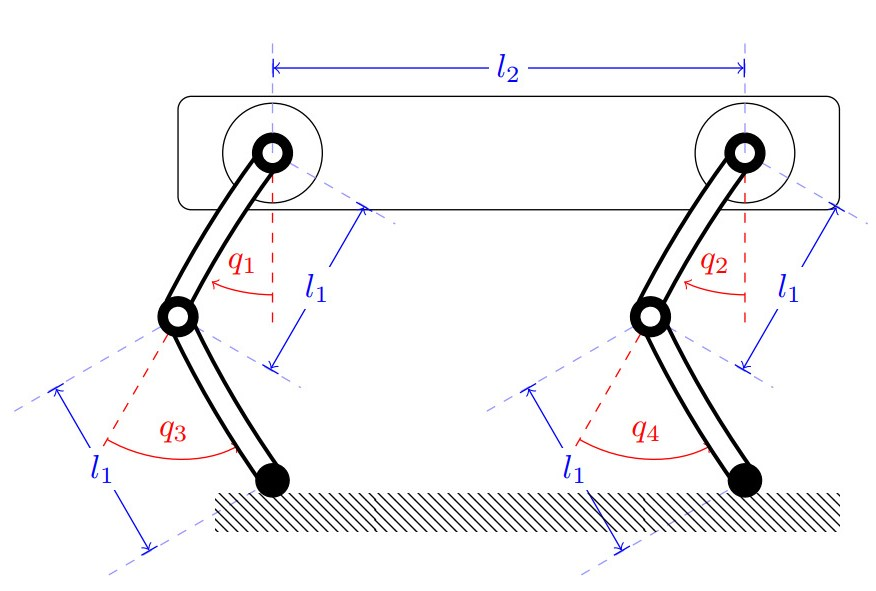
\includegraphics[scale=0.7]{images/FlatQuadruped.jpeg}
	}
	\caption{Схема плоского четвероногого робота}\label{fig:robotSagital}
\end{figure} 
Мы используем плоскую модель четвероногого робота (робот описывается в одном горизонтальном и одном вертикальном измерении), как показано на рисунке \ref{fig:robotSagital}, следуя \cite{RobotConfig}. Мы представляем его в виде пятизвенной структуры. Это позволяет нам описать положение робота с помощью семи обобщённых координат: положение и ориентация туловища робота и углов его четырёх суставов. Плоская модель объединяет ноги в пары - конфигурация обеих передних ног описывается двумя одинаковыми координатами; то же самое справедливо и для обеих задних ног. Мы обозначим как $q_1$ и $q_2$ углы, связанные с суставами, соединяющими передние и задние ноги, соответственно, а $q_3$ и $q_4$ - углы в коленных суставах передних и задних ног. Параметры робота, используемого в моделировании, приведены приведены в таблице \ref{tab:robotParam}.

\begin{table} [htbp]%
	\centering
	\caption{Параметры плоского четвероногого робота}%
	\label{tab:robotParam}% label всегда желательно идти после caption
	\renewcommand{\arraystretch}{1.5}%% Увеличение расстояния между рядами, для улучшения восприятия.
	\begin{SingleSpace}
		\begin{tabular}{@{}@{\extracolsep{20pt}}llll@{}} %Вертикальные полосы не используются принципиально, как и лишние горизонтальные (допускается по ГОСТ 2.105 пункт 4.4.5) % @{} позволяет прижиматься к краям
			\toprule     %%% верхняя линейка
			Звено & {Масса, кг} & {Длина, м} \\
			\midrule %%% тонкий разделитель. Отделяет названия столбцов. Обязателен по ГОСТ 2.105 пункт 4.4.5
			Тело   & 10     & 0.5   \\
			Переднее бедро           & 2     & 0.3   \\
			Заднее бедро        & 2     & 0.3 \\
			Передняя голень        & 2     & 0.3 \\
			Задняя голень        & 2     & 0.3  \\
			\bottomrule %%% нижняя линейка
		\end{tabular}%
	\end{SingleSpace}
\end{table}

Во время эксперимента ноги робота поддерживают контакт с землёй.
Моделирование построено следующим образом. Модель робота линеаризуется вдоль номинальной траектории, и для полученной линейной модели на каждом временном шаге путём решения уравнения Риккати находится стабилизирующий аффинный закон управления. Аналогичным образом на каждом временном шаге находятся коэффициенты усиления наблюдателя. Это представляет собой подход к планированию коэффициентов усиления при проектировании управления и наблюдателей \cite{Fromion2003}. Мы линеаризуем модель робота вокруг следующей конфигурации $q_1 =- \pi/6$, $q_2 = -\pi / 6$, $q_3 = \pi / 3$, и $q_4 = \pi / 3$.
\section{Описание эксперимента}\label{sec:ch4/sect2}
Сначала мы продемонстрируем работу предложенных методов. Мы решаем оптимизационную задачу \eqref{eq:thm1_OCP} для случая смешанной неопределённости (аддитивной и мультипликативной) и оптимизационную задачу \eqref{eq:thm3_OCP} только для мультипликативной неопределённости. Мы решаем обе задачи для различных значений $\epsilon_1$. На рисунке \ref{fig:cost} показано, как их соответствующие оптимальные затраты зависят от выбора $\epsilon_1$. Результаты показывают, что задача выполнима, а оптимальная стоимость как функция от $\epsilon_1$ описывает выпуклую кривую, что упрощает выбор оптимального значения этого параметра.

Во-вторых, мы показываем, как предложенные методы могут быть использованы для поиска наибольшего структурированного набора неопределённостей, которые может выдержать робастный линейный регулятор. Такая задача имеет ряд практических приложений. Она может быть использована для определения того, достигла ли конструкция регулятора своих пределов с точки зрения неопределённостей, которые он должен переносить. Задача также может быть решена для определения того, насколько велик набор неопределённостей, которые могут быть допустимы для данного конкретного робота и его конкретной конфигурации, что облегчает соответствующий анализ.
\section{Описание результатов эксперимента}\label{sec:ch4/sect3}